% CVPR 2025 Paper Template; see https://github.com/cvpr-org/author-kit

\documentclass[10pt,twocolumn,letterpaper]{article}

%%%%%%%%% PAPER TYPE  - PLEASE UPDATE FOR FINAL VERSION
% \usepackage{cvpr}              % To produce the CAMERA-READY version
\usepackage{cvpr}      % To produce the REVIEW version
\usepackage{subcaption}
\usepackage{multirow}
% \usepackage{hyperref}
\usepackage{amsmath}
\usepackage{amssymb}
\usepackage{mathtools}
\usepackage{amsthm}
\usepackage{algorithm, algorithmic}
\newcommand{\methodname}{\texttt{BRADD}}
% \usepackage[pagenumbers]{cvpr} % To force page numbers, e.g. for an arXiv version

% Import additional packages in the preamble file, before hyperref
\input{preamble}

% It is strongly recommended to use hyperref, especially for the review version.
% hyperref with option pagebackref eases the reviewers' job.
% Please disable hyperref *only* if you encounter grave issues, 
% e.g. with the file validation for the camera-ready version.
%
% If you comment hyperref and then uncomment it, you should delete *.aux before re-running LaTeX.
% (Or just hit 'q' on the first LaTeX run, let it finish, and you should be clear).
\definecolor{cvprblue}{rgb}{0.21,0.49,0.74}
\usepackage[pagebackref,breaklinks,colorlinks,allcolors=cvprblue]{hyperref}

%%%%%%%%% PAPER ID  - PLEASE UPDATE
\def\paperID{*****} % *** Enter the Paper ID here
\def\confName{CVPR}
\def\confYear{2025}

%%%%%%%%% TITLE - PLEASE UPDATE
\title{BRADD: \textbf{B}alancing \textbf{R}epresentations with \textbf{A}nomaly \textbf{D}etection and \textbf{D}iffusion}

%%%%%%%%% AUTHORS - PLEASE UPDATE
\author{Filipe Laitenberger\\
University of Amsterdam\\
Netherlands\\
{\tt\small filipe.laitenberger@student.uva.nl}\\
\and
Nesta Midavaine\\
University of Amsterdam\\
Netherlands\\
\and
Ioana Simion\\
University of Amsterdam\\
Netherlands\\
\and
Stefan Vasilev\\
University of Amsterdam\\
Netherlands\\
\and
Hirokatsu Kataoka\\
AIST / University of Oxford\\
Japan / United Kingdom\\
\and
Cees G. M. Snoek\\
University of Amsterdam\\
Netherlands\\
\and
Yuki M Asano\\
University of Technology Nuremberg\\
Germany\\
\and
Mohammadreza Salehi\\
University of Amsterdam\\
Netherlands\\
% For a paper whose authors are all at the same institution,
% omit the following lines up until the closing ``}''.
% Additional authors and addresses can be added with ``\and'',
% just like the second author.
% To save space, use either the email address or home page, not both
}

\begin{document}
\maketitle

\begin{abstract}
Self-supervised learning (SSL) has allowed for advancements in language processing and computer vision, as unlabelled data is available in large quantities. However, imbalances in training datasets can lead to strong biases in the learned features of pre-trained models. Previous results show that pre-training using imbalanced data can also hurt downstream performance. We propose a data-centric approach: our method trains on the data, finds underrepresented samples, and uses diffusion to generate novel data complementing the underrepresented images. Our proposed method, BRADD (Balancing Representations through Anomaly Detection and Diffusion), utilizes distance-based outlier detection to identify regions of the embedding space that are underrepresented in each training cycle. Experimental results on ImageNet-100-LT demonstrate that BRADD consistently outperforms both balanced and imbalanced baselines, with significant improvements on fine-grained classification tasks. Detailed ablation studies confirm that both out-of-distribution sample selection and diffusion-based generation contribute substantially to the effectiveness of our approach, offering a promising alternative to model-centric solutions for addressing imbalance in self-supervised learning.
\end{abstract}    
\section{Introduction}
\label{sec:intro}

Self-supervised learning (SSL) methods have emerged as powerful techniques for learning transferable features across diverse tasks~\cite{chen2020simple, DINO, oquab2023dinov2}. However, their performance is significantly affected by dataset imbalance~\cite{assran2210hidden, tian2021divide, ts}. For instance, SimCLR underperforms on long-tailed datasets due to insufficient negative samples~\cite{tian2021divide}, while joint-embedding methods like VICReg assume uniform clustering, hampering performance on imbalanced data~\cite{assran2210hidden}.

Existing solutions typically adopt model-centric approaches, such as ensemble learning~\cite{tian2021divide}, incorporating arbitrary feature priors~\cite{assran2210hidden}, or modifying training dynamics~\cite{ts}. These approaches, however, often require prior knowledge of dataset distributions or extensive hyperparameter tuning, contradicting the unsupervised nature of SSL.

We propose BRADD (\textbf{B}alancing \textbf{R}epresentations with \textbf{A}nomaly \textbf{D}etection and \textbf{D}iffusion), a data-centric approach to address imbalance in SSL. BRADD divides training into cycles, identifies underrepresented samples via OOD detection after each cycle, and augments them using diffusion models for subsequent training. This approach (1) eliminates the need for prior dataset knowledge and (2) dynamically balances the latent space to avoid suboptimal local minima.

Experiments on ImageNet-100-LT across multiple architectures (ResNet-50, ViT-S, ViT-B) and SSL methods (SimCLR, DINO, MoCo) demonstrate that BRADD consistently outperforms both balanced and imbalanced baselines on diverse downstream tasks. BRADD achieves significant improvements on fine-grained tasks (up to 11.7\% on Oxford Flowers) and surpasses state-of-the-art methods on CIFAR-10 (73.3\%) and CIFAR-100 (45.4\%), showing that our data-centric approach offers a promising alternative to model-centric solutions.
\section{Related Work}
\label{sec:related-work}

\noindent
\textbf{Self-Supervised Learning (SSL)} leverages unlabeled data to learn meaningful representations for downstream tasks. In computer vision, three main approaches are: (1) masked prediction \cite{he2022masked}, (2) contrastive learning like MoCo \cite{he2020momentum} and SimCLR \cite{chen2020simple}, and (3) self-distillation methods such as DINO \cite{DINO}. These techniques have enabled large-scale training of models with emergent abilities \cite{wei2022emergent}.

\noindent
\textbf{Training on Imbalanced Datasets} often leads to inferior performance and bias toward majority classes \cite{johnson2019survey}. While SSL methods are more robust to imbalance than supervised approaches \cite{liu2021self}, they still exhibit diminished performance on imbalanced data. Current solutions are primarily model-centric, attempting to learn arbitrary feature priors \cite{assran2210hidden}. Data-centric approaches that directly complement imbalanced datasets remain underexplored.

\noindent
\textbf{Out-Of-Distribution (OOD) Detection} is crucial for enhancing model robustness by maintaining high-quality datasets \cite{whang2023data}. Distance-based approaches \cite{sun2022out} identify OOD samples by measuring their distance from in-distribution samples in the embedding space. These non-parametric methods offer flexibility without distributional assumptions, making them suitable for imbalanced, unlabeled data.

\noindent
\textbf{Diffusion-Based Image Generation} models systematically add and then remove noise to generate high-quality images \cite{ho2020denoising}. Stable Diffusion \cite{rombach2022highresolution}, particularly Stable Diffusion 2 UnClip, leverages CLIP embeddings to generate semantically similar images to the input context. Its ability to perform image-to-image generation while preserving semantic content makes it well-suited for augmenting self-supervised learning datasets.
\section{Method: BRADD}
\label{sec:method}

\begin{figure*}[h]
    \centering
    
\includegraphics[width=0.7\textwidth]{Images/BRIDGE.pdf}
    \captionsetup[subfigure]{skip=0pt}
    \caption{The BRADD algorithm augments the most underrepresented datapoints in a dataset based on OOD detection.}
    \label{fig:full_pipeline}
\end{figure*}

We propose BRADD (Balancing Representations with Anomaly Detection and Diffusion), a data-centric approach to address imbalance in self-supervised learning. Unlike model-centric approaches, BRADD identifies and augments underrepresented concepts in the data distribution itself.

\begin{algorithm}[h]
\caption{BRADD: Balancing Representations through Anomaly Detection and Diffusion}
\label{alg:bradd}
\begin{algorithmic}[1]
\STATE {\bfseries Input:} model $m$, SSL algorithm $a$, diffusion model $m_d$, cycles $N_C$, epochs per cycle $N_E$, dataset $D$, samples per point $N_{Aug}$, OOD samples $N_{OOD}$
\REPEAT
\STATE Train $m$ using $a$ for $N_E$ epochs on $D$
\STATE Compute embeddings $E = \{m(x_i) | x_i \in D\}$
\STATE Find OOD points $O = \{x_i | \text{rank}(d_{kNN}(m(x_i), E)) \leq N_{OOD}\}$
\FOR{$x \in O$}
\STATE $D = D \cup \{m_d(x, \epsilon_j) | j = 1,...,N_{Aug}\}$
\ENDFOR
\UNTIL{$N_C$ cycles completed}
\end{algorithmic}
\end{algorithm}

\noindent
BRADD alternates between self-supervised pre-training and dataset augmentation phases (Algorithm \ref{alg:bradd}). After training for $N_E$ epochs, we identify underrepresented data points by computing k-nearest neighbor distances in the embedding space. Rather than using a percentile threshold, we select the top-$N_{OOD}$ samples with highest k-NN distances, providing precise control over augmentation.

\noindent
For each identified OOD point, we generate $N_{Aug}$ new samples using Stable Diffusion 2 UnCLIP \cite{rombach2021highresolution}, which preserves semantic content while introducing sufficient variation. We use k=5 for k-NN computation, $N_{OOD}=500$, and $N_{Aug}=5$, adding 2,500 new images per cycle across 5 cycles with 20 epochs each (100 total epochs).
\section{Experiments}
\label{experiments}


\input{Tables/baseline_comp}

\begin{table*}[t]
\centering
\setlength{\tabcolsep}{2pt}
\caption{\centering \textbf{Comparison to SOTA}\\(ResNet50, SimCLR, ImageNet-100-LT, 500 epochs)}
{\begin{tabular}{l cc cc cc cc cc cc}
    \toprule
     & \multicolumn{2}{c}{\textbf{C-10}} &  \multicolumn{2}{c}{\textbf{C-100}}  &  \multicolumn{2}{c}{\textbf{Cars}} &  \multicolumn{2}{c}{\textbf{Aircraft}} &  \multicolumn{2}{c}{\textbf{Flowers}} &  \multicolumn{2}{c}{\textbf{Pets}} \\
     \cmidrule(r){2-3}
     \cmidrule(l){4-5}
     \cmidrule(l){6-7}
     \cmidrule(l){8-9}
     \cmidrule(l){10-11}
     \cmidrule(l){12-13}
    Method & Lin. & KNN & Lin. & KNN & Lin. & KNN & Lin. & KNN & Lin. & KNN & Lin. & KNN \\
    \midrule
    
     \multirow{1}{*}{SDCLR \cite{sdclr}}        & 68.72   &  65.16 & 38.71 & 35.53 & 7.84 & 5.21 & 11.24 & 10.11 & 11.87 & 31.14 & 40.22 & 21.98 \\
    \multirow{1}{*}{TS \cite{ts}}    & 71.26 &  \textbf{66.76} & 43.90 & \textbf{35.64} & \textbf{10.91} & \textbf{5.58} & \textbf{12.95} & \textbf{10.85} & 32.05 & 3.36 & \textbf{47.01} & \textbf{23.20} \\
    \multirow{1}{*}{BRADD (ours)}     & \textbf{73.34}  &  61.76 & \textbf{45.38} & 32.26 & 8.95 & 4.73 & 10.95 & 7.92 & 26.14 & 24.94 & 34.68 & 16.05 \\
    \bottomrule
\end{tabular}
\label{table:sota_comp}}
\end{table*}

\begin{table*}[t]
\centering
\setlength{\tabcolsep}{2pt}
\caption{\centering \textbf{Comparison to SOTA}\\(ResNet50, SimCLR, ImageNet-100-LT, 800 epochs, reporting mean acc. across three different runs)}
{\begin{tabular}{l cc cc cc cc cc cc cc cc cc}
    \toprule
     & \multicolumn{2}{c}{\textbf{C-10}} &  \multicolumn{2}{c}{\textbf{C-100}}  &  \multicolumn{2}{c}{\textbf{Cars}} &  \multicolumn{2}{c}{\textbf{Aircraft}} &  \multicolumn{2}{c}{\textbf{Flowers}} &  \multicolumn{2}{c}{\textbf{Pets}} & \multicolumn{2}{c}{\textbf{IN-100-LT}} \\
     \cmidrule(r){2-3}
     \cmidrule(l){4-5}
     \cmidrule(l){6-7}
     \cmidrule(l){8-9}
     \cmidrule(l){10-11}
     \cmidrule(l){12-13}
     \cmidrule(l){14-15}
    Method & Lin.\ & KNN & Lin.\ & KNN & Lin.\ & KNN & Lin.\ & KNN & Lin.\ & KNN & Lin.\ & KNN & Lin.\ & KNN \\
    \midrule
    \multirow{1}{*}{SimCLR}              & 72.80 & 62.03 & 44.12 & 29.08 &  9.23 &  3.50 & 11.36 &  7.19 & 31.81 & 20.57 & 35.14 & 15.85 & \textemdash & \textemdash \\
    \multirow{1}{*}{TS (T=100)}          & 68.59 & 55.31 & 37.13 & 21.48 &  6.05 &  2.11 &  8.98 &  4.70 & 22.66 & 13.64 & 31.71 & 13.60 & \textemdash & \textemdash \\   
    \multirow{1}{*}{TS (T=400)}          & 68.16 & 55.41 & 37.65 & 21.38 &  5.64 &  2.39 &  9.46 &  4.55 & 25.71 & 13.60 & 32.07 & 13.65 & \textemdash & \textemdash \\
    \multirow{1}{*}{BRIDGE}              & 74.29 & 62.71 & 46.87 & 30.49 & 11.03 &  4.54 & 12.98 &  7.89 & 37.69 & 24.08 & 38.30 & 17.63 & \textemdash & \textemdash \\
    \multirow{1}{*}{BRIDGE + TS (T=400)} & 66.45 & 50.92 & 35.61 & 18.88 &  5.31 &  1.62 &  8.08 &  3.50 & 19.39 & 11.11 & 27.46 & 12.68 & \textemdash & \textemdash \\
    \multirow{1}{*}{SDCLR}               & 49.97 & 40.99 &  8.64 & 14.01 &  0.65 &  1.27 &  1.07 &  2.86 &  1.31 &  6.67 &  4.07 &  5.85 & 14.83 & 40.92 \\
    \bottomrule
\end{tabular}}
\label{table:sota_comp}
\end{table*}


\begin{table*}[t]
\centering
\setlength{\tabcolsep}{2pt}
\caption{\centering \textbf{Comparison to SOTA}\\(ResNet50, SimCLR, ImageNet-100-LT, 800 epochs, 3 different runs)}
{\begin{tabular}{l cc cc cc cc cc cc}
    \toprule
     & \multicolumn{2}{c}{\textbf{C-10}} &  \multicolumn{2}{c}{\textbf{C-100}}  &  \multicolumn{2}{c}{\textbf{Cars}} &  \multicolumn{2}{c}{\textbf{Aircraft}} &  \multicolumn{2}{c}{\textbf{Flowers}} &  \multicolumn{2}{c}{\textbf{Pets}} \\
     \cmidrule(r){2-3}
     \cmidrule(l){4-5}
     \cmidrule(l){6-7}
     \cmidrule(l){8-9}
     \cmidrule(l){10-11}
     \cmidrule(l){12-13}
    Method & Lin.\ & KNN & Lin.\ & KNN & Lin.\ & KNN & Lin.\ & KNN & Lin.\ & KNN & Lin.\ & KNN \\
    \midrule
    \multirow{1}{*}{SimCLR}        & 69.89 & 36.31 & 40.92 & 11.34 &  8.62 &  1.37 & 11.22 &  2.45 & 30.72 &  6.35 & 35.68 &  5.91 \\
    \multirow{1}{*}{TS}    & 66.56 & 33.92 & 36.42 & 10.06 &  6.00 &  1.31 &  9.01 &  2.72 & 26.58 &  5.32 & 33.79 &  5.79 \\
    \bottomrule
\end{tabular}}
\label{table:sota_comp}
\end{table*}

\input{Tables/ablations}


%
%\begin{figure*}[htbp]
%   \centering
%   \begin{subfigure}[b]{0.3\textwidth}
%       \centering
%       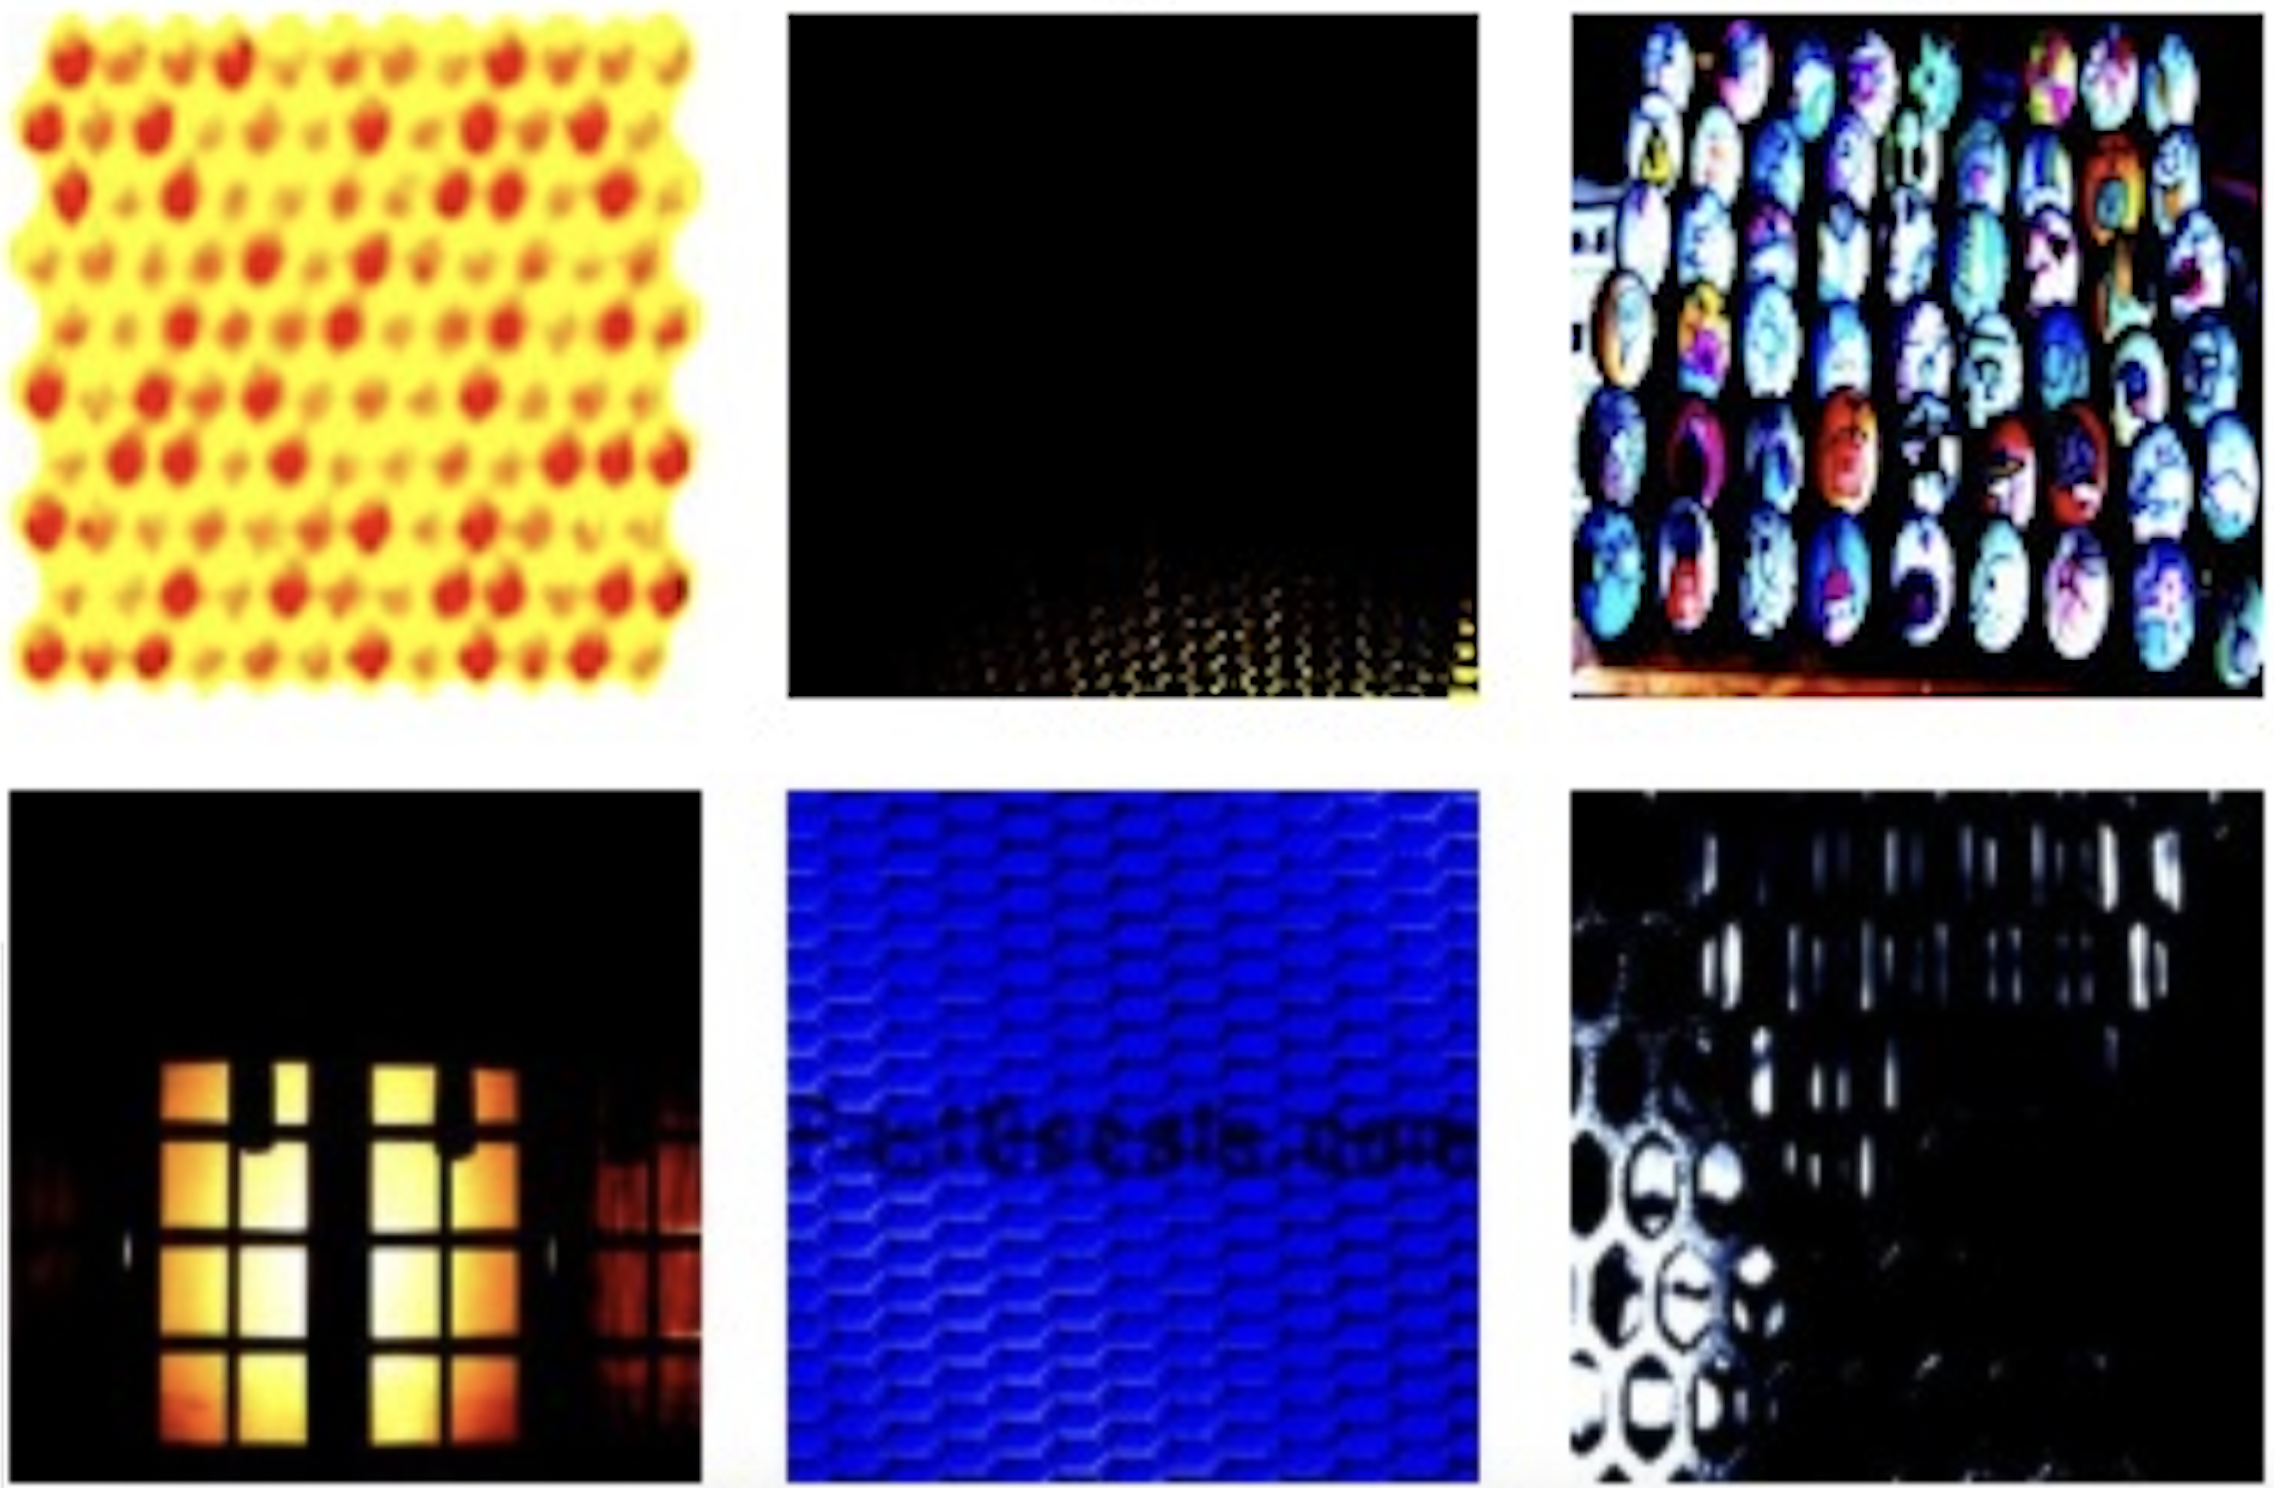
\includegraphics[width=\textwidth]{Images/most-ood-images-cycle 1.png}
%       \caption{Most OOD images after cycle 1}
%       \label{fig:most-ood-images-1}
%   \end{subfigure}
%   \hfill
%   \begin{subfigure}[b]{0.3\textwidth}
%       \centering
%       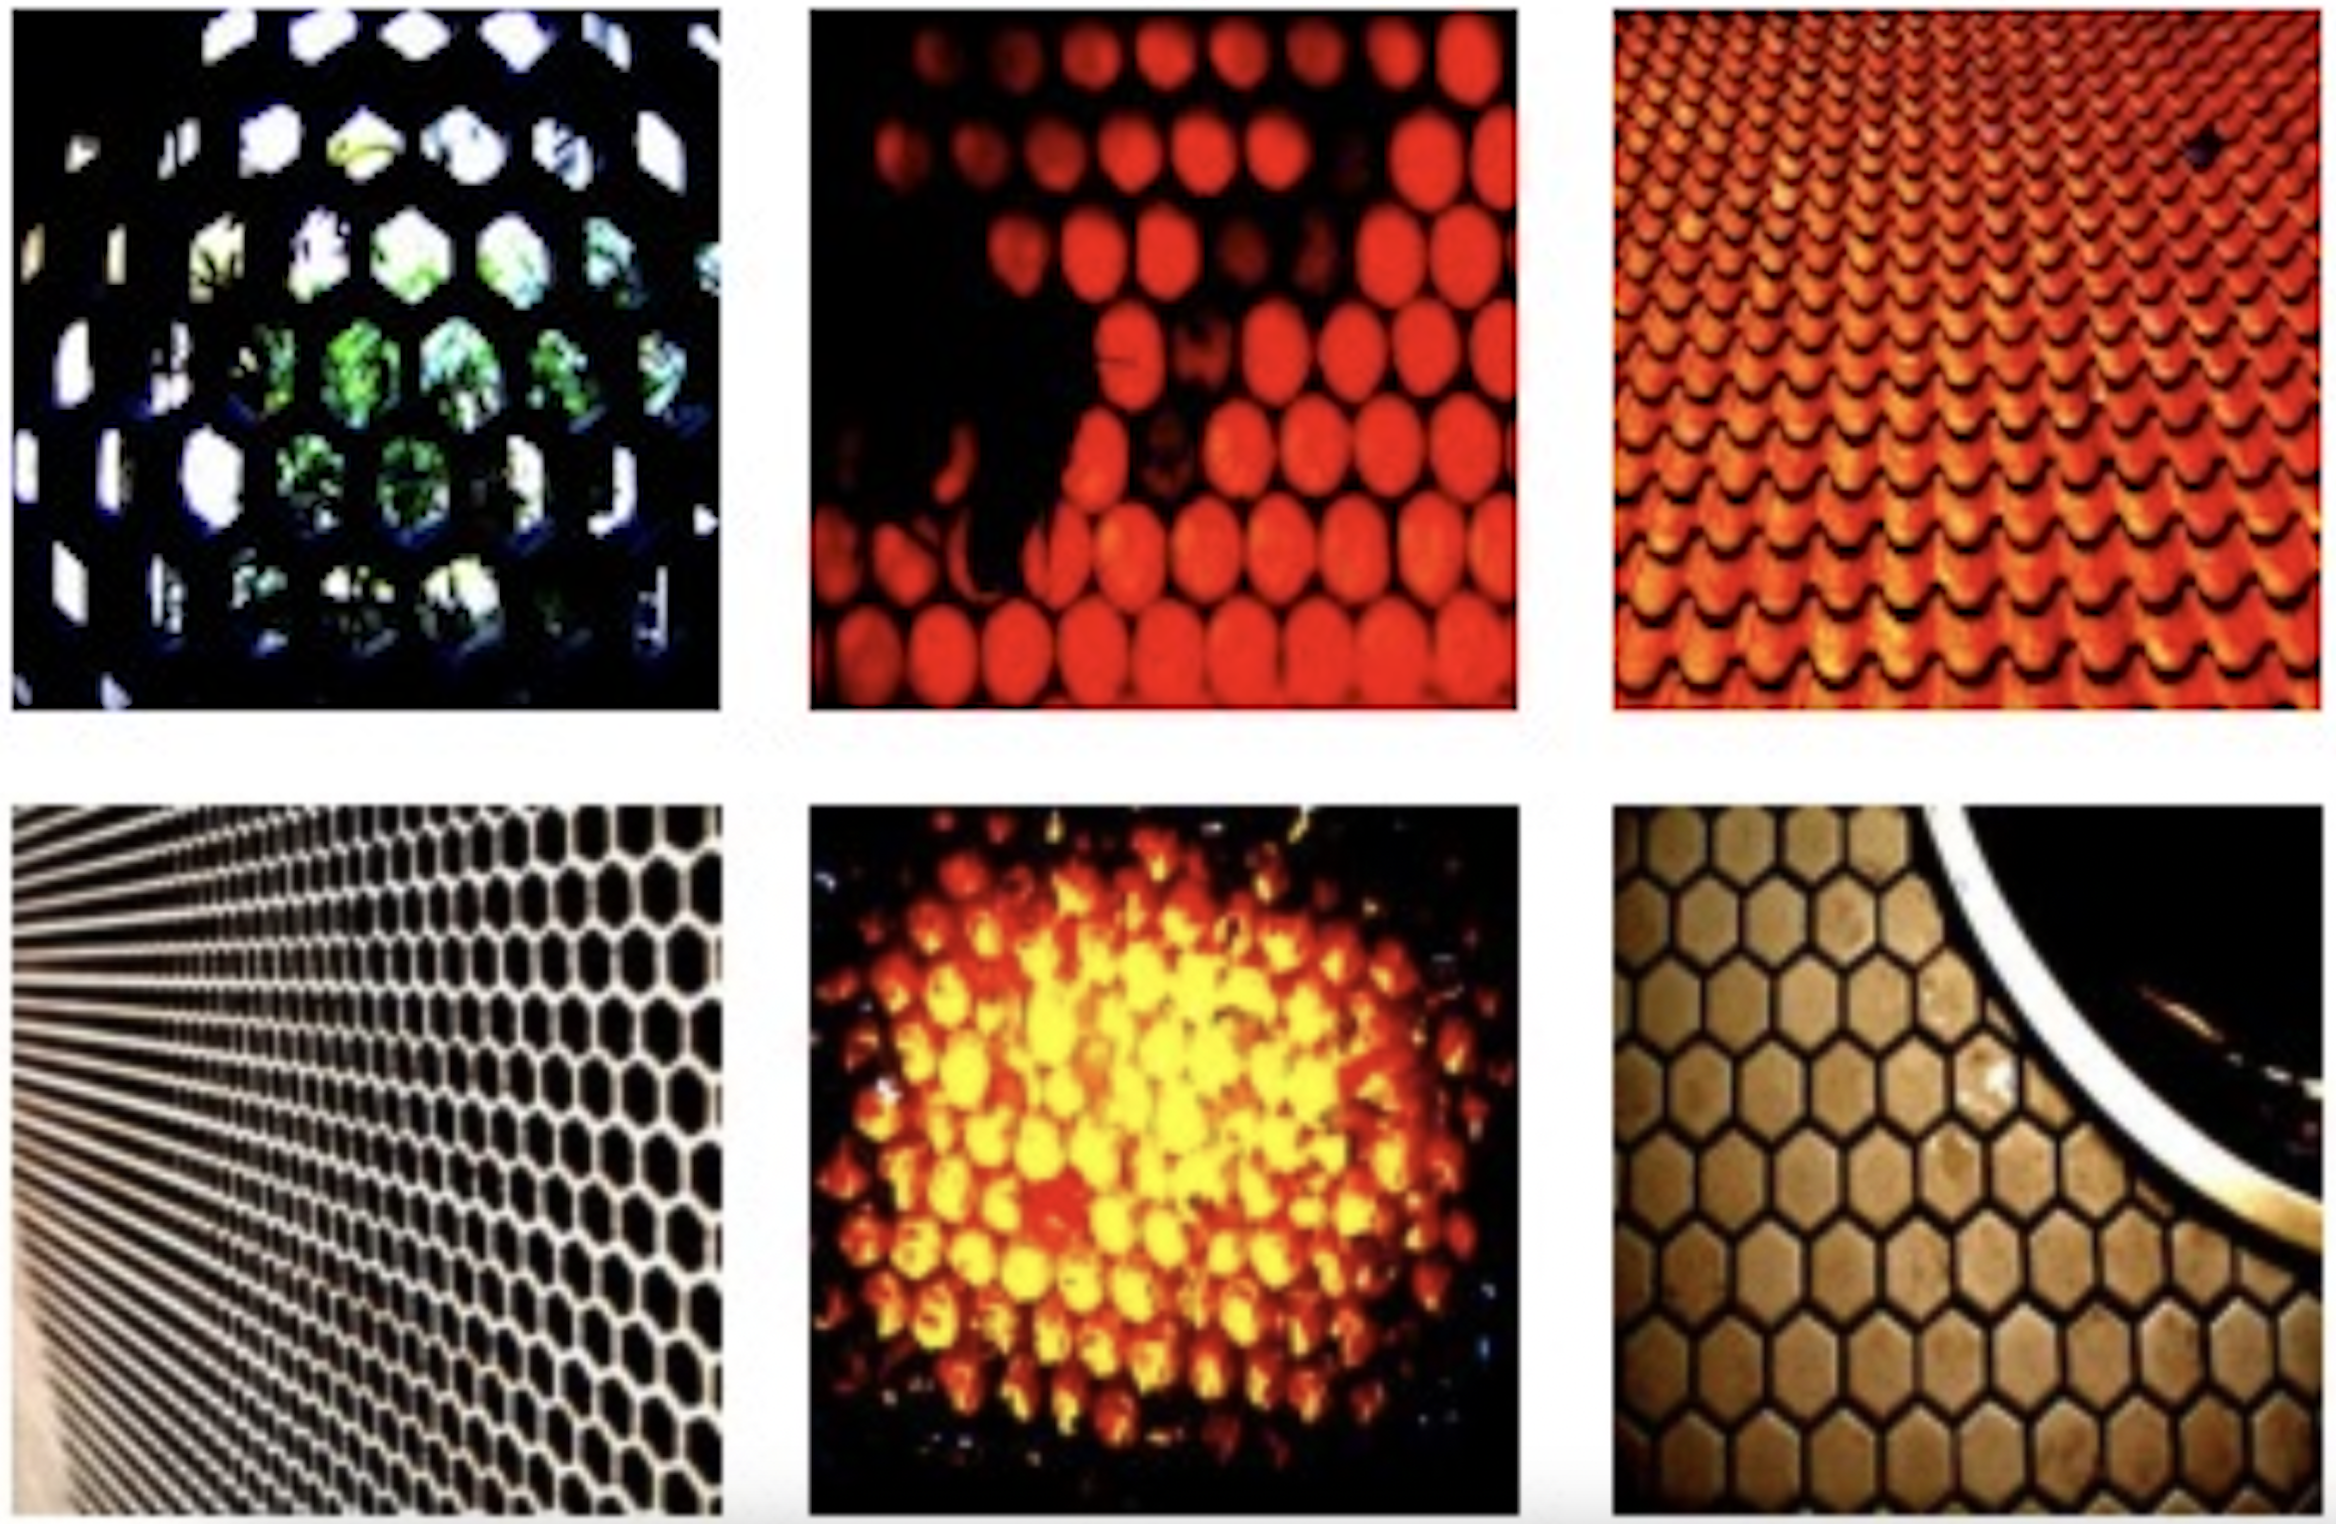
\includegraphics[width=\textwidth]{Images/most-ood-images-cycle 2.png}
%       \caption{Most OOD images after cycle 2}
%       \label{fig:most-ood-images-2}
%   \end{subfigure}
%   \hfill
%   \begin{subfigure}[b]{0.3\textwidth}
%       \centering
%       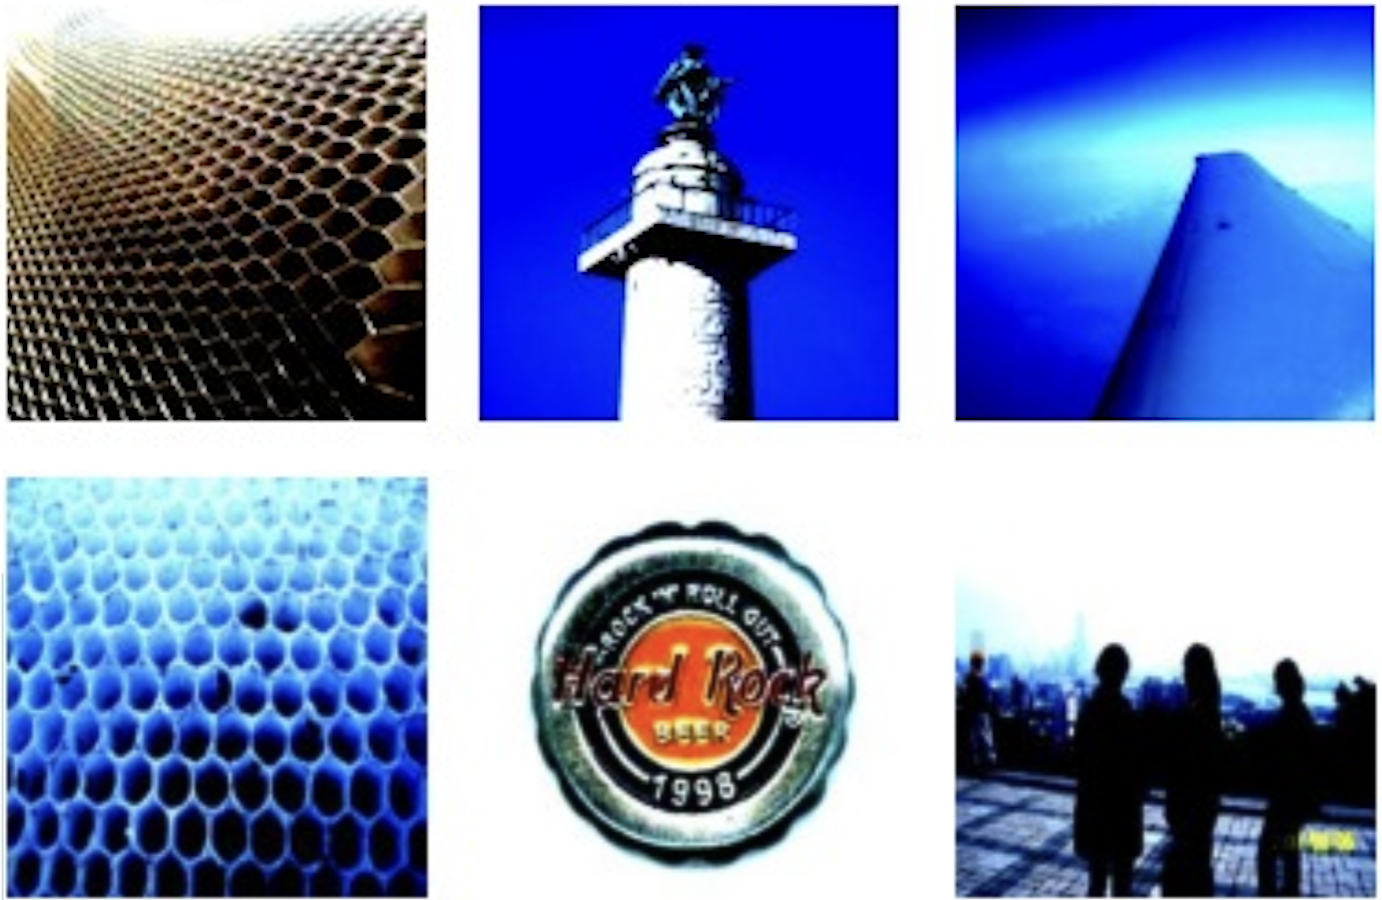
\includegraphics[width=\textwidth]{Images/most-ood-images-cycle 3.png}
%       \caption{Most OOD images after cycle 3}
%       \label{fig:most-ood-images-3}
%   \end{subfigure}
%   \caption{The characteristics of the detected OOD datapoints change over time, commencing as strange patterns and over time turning into much more mundane objects.}
%   \label{fig:most-ood-images}
%\end{figure*}
%

\noindent
To evaluate the performance of our proposed method BRADD (Balancing Representations through Automated Detection and Diffusion), we conduct experiments on ImageNet-100-LT. We test various backbone architectures, SSL methods, and implementation details through comprehensive ablation studies, and compare against state-of-the-art approaches.

\subsection{ImageNet-100 Experiments}

\noindent
ImageNet-100 is a subset of ImageNet with 100 randomly selected classes \cite{tian2020contrastive}. Following previous work \cite{imagenet-lt}, we introduce imbalance by creating a long-tailed distribution (ImageNet-100-LT) that follows a Pareto distribution with $\alpha=6$. The dataset contains around 15 thousand images.\\
\noindent
\textbf{Models.} We evaluate our method across multiple architectures: ResNet-50 (25.6M parameters), ViT-Small (22.1M parameters), and ViT-Base (86.6M parameters).\\
\noindent
\textbf{Self-Supervised Learning Methods.} Our primary experiments use SimCLR \cite{chen2020simple} with a temperature of 0.5, and we later compare with DINO \cite{DINO} and MoCo \cite{moco} in our ablation studies.\\
\noindent
\textbf{Downstream Evaluation.} We evaluate the learned features using both linear probing and K-nearest neighbor (KNN) classification across multiple datasets: CIFAR-10, CIFAR-100 \cite{krizhevsky2009learning}, Stanford Cars \cite{cars}, FGVC Aircraft \cite{aircraft}, Oxford Flowers \cite{flowers}, and Oxford-IIIT Pets \cite{pets}.\\
\noindent
\textbf{Baselines.} We train two baselines: (1) a model trained on a balanced subset of ImageNet-100 with as much data uniformly removed as in ImageNet-100-LT and (2) a model trained on the imbalanced ImageNet-100-LT.\\
\noindent
\textbf{Proposed Method.} Our proposed method BRADD starts with ImageNet-100-LT and trains for multiple cycles, where each cycle consists of training epochs followed by OOD detection and generation steps.
\subsection{Experimental Results}
\noindent
Table \ref{table:baseline_comp} compares our method against balanced and imbalanced baselines using a ViT-B backbone with SimCLR. The results demonstrate that:
\begin{itemize}
\item While imbalance causes only slight performance degradation compared to the balanced setting on some datasets, our method consistently outperforms both baselines across all datasets.
\item BRADD achieves substantial improvements in linear probing, with gains of up to 11.72\% on Oxford Flowers and 7.53\% on Oxford-IIIT Pets compared to the imbalanced baseline.
\item Our method also shows consistent improvements in KNN classification, demonstrating the enhanced quality of the learned feature space.
\end{itemize}
\noindent
Table \ref{table:sota_comp} shows BRADD compared to state-of-the-art methods using ResNet-50 with SimCLR (500 epochs):
\begin{itemize}
\item Our method achieves superior linear probing performance on CIFAR-10 (73.34\%) and CIFAR-100 (45.38\%) compared to previous methods.
\item While TS \cite{ts} performs better on KNN classification for most datasets, BRADD shows competitive performance across all benchmarks.
\end{itemize}
\subsection{Ablation Studies}
\noindent
To analyze the effectiveness of different components in our approach, we conducted extensive ablation studies:\\
\noindent
\textbf{SSL Method.} Table \ref{table:pretraining-abl} demonstrates that SimCLR consistently outperforms DINO and MoCo across all datasets when using our method, with substantial margins particularly on fine-grained classification tasks.\\
\noindent
\textbf{Backbone Architecture.} As shown in Table \ref{table:backbone_abl}, we compared ViT-S, ViT-B, and ResNet-50 backbones. ResNet-50 achieves the best linear probing performance on CIFAR-10 (71.17\%), while ViT architectures perform better on fine-grained datasets, with ViT-B showing the strongest performance on Oxford-IIIT Pets (30.08\%).\\
\noindent
\textbf{Sample Selection Strategy.} In Table \ref{table:sample_selection}, we compare uniform sampling versus our OOD-based selection. The results confirm that OOD-based selection provides consistent performance gains, validating our hypothesis that targeting underrepresented regions of the feature space is more effective than random augmentation.\\
\noindent
\textbf{Sample Generation Method.} Table \ref{table:sample_generation} compares re-population (adding back removed samples) versus generation using Stable Diffusion. While both approaches improve over the baseline, Stable Diffusion generation yields better results, particularly on fine-grained datasets like Oxford Flowers.\\
\noindent
\textbf{Number of Cycles.} As shown in Table \ref{table:n_cycle_abl}, we tested different numbers of cycles (2, 5, 10, 20) while keeping the total number of generated images fixed. Performance generally improves with more cycles, with the best results at 20 cycles for CIFAR-10 (68.68\% linear probing accuracy) and 5 cycles for Oxford-IIIT Pets (30.08\%).\\\
\noindent
\textbf{Number of OOD Samples.} Table \ref{table:n_samples_abl} analyzes the effect of selecting different numbers of samples per cycle for augmentation. We find that 500 samples per cycle provides the optimal balance, while selecting too many samples (2500) degrades performance, suggesting that focusing on the most out-of-distribution samples is important.
\section{Conclusion}
Our comprehensive experiments demonstrate that BRADD effectively mitigates the negative impact of dataset imbalance in self-supervised learning. By strategically detecting regions of the feature space that are underrepresented and augmenting them with generated samples, our method achieves consistent improvements across different architectures, SSL methods, and downstream tasks. The ablation studies confirm that both OOD-based sample selection and diffusion-based generation contribute significantly to the effectiveness of our approach.
{
    \small
    \bibliographystyle{ieeenat_fullname}
    \bibliography{main}
}

% WARNING: do not forget to delete the supplementary pages from your submission 
% \clearpage
\setcounter{page}{1}
\maketitlesupplementary


\section{Theoretical Foundations for BRIDGE}\label{app:theory}

\noindent
To formalize the problem of imbalanced representation learning, we introduce several key definitions and theorems.

\begin{definition}[Image and Dataset Spaces]
Let $\mathcal{X}$ be the space of all possible images, and $D = \{x_1, x_2, \ldots, x_n\} \subset \mathcal{X}$ be our finite dataset.
\end{definition}

\begin{definition}[Concepts]
Let $\mathcal{C} = \{C_1, C_2, \ldots, C_m\}$ be a partition of $\mathcal{X}$ representing distinct semantic concepts, where each $C_i \subset \mathcal{X}$. We denote the restriction of dataset $D$ to concept $C_i$ as $D_i = D \cap C_i$.
\end{definition}

\begin{definition}[Information Density]
The information density $\mathcal{I}(C_i)$ of a concept $C_i$ is defined as the minimum number of examples needed to represent it effectively. Formally:
\begin{equation}
\mathcal{I}(C_i) = \min\{|S| : S \subset C_i \text{ and } \mathcal{L}(f_S, C_i) \leq \epsilon\}
\end{equation}
where $f_S$ is a representation learned from subset $S$, and $\mathcal{L}(f_S, C_i)$ is a loss function measuring how well $f_S$ represents concept $C_i$.
\end{definition}

\begin{definition}[Balanced Dataset]
A dataset $D$ is $\delta$-balanced with respect to concepts $\mathcal{C}$ if for all concepts $C_i \in \mathcal{C}$:
\begin{equation}
\frac{|D_i|}{\mathcal{I}(C_i)} \geq \delta
\end{equation}
where $\delta \in (0,1]$ is a balance factor. When $\delta = 1$, the dataset has sufficient examples for each concept.
\end{definition}

\begin{assumption}[Ideal Embedding]
\label{assump:ideal}
In our initial analysis, we assume that the encoder $f_\theta$ perfectly clusters images by concepts. Formally, there exists a distance threshold $\tau$ such that:
\begin{align}
\forall x_i \in C_i, x_j \in C_j: \|f_\theta(x_i) - f_\theta(x_j)\|_2 < \tau \iff i = j
\end{align}
\end{assumption}

\begin{theorem}[Embedding Density Reflects Concept Representation]
\label{thm:density}
Under Assumption \ref{assump:ideal}, for any two concepts $C_i$ and $C_j$ with $|D_i|/\mathcal{I}(C_i) < |D_j|/\mathcal{I}(C_j)$, the average k-NN distance for points in $D_i$ is greater than for points in $D_j$:
\begin{equation}
\mathbb{E}_{x \in D_i}[d_{kNN}(f_\theta(x), Z)] > \mathbb{E}_{x \in D_j}[d_{kNN}(f_\theta(x), Z)]
\end{equation}
\end{theorem}

\begin{proof}
Under Assumption \ref{assump:ideal}, embeddings form distinct clusters by concept. Let $Z_i = \{f_\theta(x) : x \in D_i\}$ be the set of embeddings for concept $C_i$. For any $x \in D_i$, its k nearest neighbors must come from the same concept, i.e., from $Z_i$, since the distance to points from other concepts exceeds $\tau$ while distances within the same concept are less than $\tau$.

\noindent
For points uniformly distributed in a d-dimensional space of volume $V$, the expected distance to the k-th nearest neighbor of a random point scales as $\mathcal{O}(V^{1/d} \cdot n^{-1/d})$, where $n$ is the number of points. This scaling relationship follows from the fact that the expected distance between uniformly distributed points in a region of volume $V$ is proportional to $V^{1/d}$, and with $n$ points, the average volume per point is $V/n$.

\noindent
The embeddings of concept $C_i$ occupy a region in the embedding space with some effective volume $V_i$. Since $|Z_i| = |D_i|$, the average k-NN distance for points in $D_i$ scales as:
\begin{equation}
\mathbb{E}_{x \in D_i}[d_{kNN}(f_\theta(x), Z_i)] \propto V_i^{1/d} \cdot |D_i|^{-1/d}
\end{equation}

\noindent
Assuming similar volumes for the concept regions (i.e., $V_i \approx V_j$), we have:
\begin{equation}
\frac{\mathbb{E}_{x \in D_i}[d_{kNN}(f_\theta(x), Z_i)]}{\mathbb{E}_{x \in D_j}[d_{kNN}(f_\theta(x), Z_j)]} \propto \left(\frac{|D_j|}{|D_i|}\right)^{1/d}
\end{equation}

\noindent
Given that $|D_i|/\mathcal{I}(C_i) < |D_j|/\mathcal{I}(C_j)$, and assuming comparable information densities, we have $|D_i| < |D_j|$. Therefore:
\begin{equation}
\begin{aligned}
\mathbb{E}_{x \in D_i}[d_{kNN}(f_\theta(x), Z)] &= \mathbb{E}_{x \in D_i}[d_{kNN}(f_\theta(x), Z_i)] \\
&> \mathbb{E}_{x \in D_j}[d_{kNN}(f_\theta(x), Z_j)] \\
&= \mathbb{E}_{x \in D_j}[d_{kNN}(f_\theta(x), Z)]
\end{aligned}
\end{equation}
\end{proof}

\begin{theorem}[Rank-Based Selection Identifies Underrepresented Concepts]
\label{thm:rank}
Let $O = \{x_i \in D : \text{rank}(d_{kNN}(f_\theta(x_i), Z)) \leq N_{OOD}\}$ be the set of $N_{OOD}$ points with the highest k-NN distances. Under Assumption \ref{assump:ideal}, $O$ contains a higher proportion of points from underrepresented concepts than from well-represented concepts:
\begin{equation}
\frac{|O \cap D_i|}{|D_i|} > \frac{|O \cap D_j|}{|D_j|} \text{ for } \frac{|D_i|}{\mathcal{I}(C_i)} < \frac{|D_j|}{\mathcal{I}(C_j)}
\end{equation}
\end{theorem}

\begin{proof}
From Theorem \ref{thm:density}, points from underrepresented concepts have higher expected k-NN distances. Let $F_i(d)$ be the cumulative distribution function (CDF) of k-NN distances for points in concept $C_i$, i.e., $F_i(d) = \Pr(d_{kNN}(f_\theta(x), Z) \leq d | x \in D_i)$.

\noindent
Under Assumption \ref{assump:ideal} and the uniform distribution assumption within concept regions, the CDF $F_i(d)$ is determined by the point density in the concept region. For concepts $C_i$ and $C_j$ with $|D_i|/\mathcal{I}(C_i) < |D_j|/\mathcal{I}(C_j)$, the lower density of points in concept $C_i$ results in $F_i(d) < F_j(d)$ for all distance thresholds $d$.

\noindent
When selecting the top $N_{OOD}$ points by k-NN distance, there exists some distance threshold $d^*$ such that points with $d_{kNN}(f_\theta(x), Z) > d^*$ are selected. The proportion of points selected from concept $C_i$ is:
\begin{equation}
\frac{|O \cap D_i|}{|D_i|} = 1 - F_i(d^*)
\end{equation}

\noindent
Similarly, for concept $C_j$:
\begin{equation}
\frac{|O \cap D_j|}{|D_j|} = 1 - F_j(d^*)
\end{equation}

\noindent
Since $F_i(d^*) < F_j(d^*)$, we have:
\begin{equation}
\frac{|O \cap D_i|}{|D_i|} = 1 - F_i(d^*) > 1 - F_j(d^*) = \frac{|O \cap D_j|}{|D_j|}
\end{equation}

\noindent
Therefore, underrepresented concepts are proportionally more represented in the selected set $O$.
\end{proof}

\begin{assumption}[Ideal Diffusion]
\label{assump:diffusion}
The diffusion model $g: \mathcal{X} \times \mathbb{R}^r \rightarrow \mathcal{X}$ generates samples that belong to the same concept as the input:
\begin{equation}
\forall x \in C_i, \epsilon \sim \mathcal{N}(0, I_r): g(x, \epsilon) \in C_i
\end{equation}
\end{assumption}

\begin{theorem}[Augmentation Improves Balance]
\label{thm:augment}
Let $D' = D \cup \{g(x, \epsilon_{j,x}) : x \in O, j \in \{1,\ldots,N_{Aug}\}\}$ where $O$ is the set of $N_{OOD}$ points with highest k-NN distances in $Z$, and $N_{Aug}$ is the number of augmentations per point. Under Assumptions \ref{assump:ideal} and \ref{assump:diffusion}, if $N_{OOD}$ and $N_{Aug}$ are sufficiently large, then $D'$ has a higher balance factor than $D$.
\end{theorem}

\begin{proof}
\noindent
From Theorem \ref{thm:rank}, points in $O$ come disproportionately from underrepresented concepts. Let $p_i = |O \cap D_i|/|O|$ be the proportion of points in $O$ from concept $C_i$.

\noindent
Under Assumption \ref{assump:diffusion}, for each $x \in O \cap D_i$, all generated samples $g(x, \epsilon)$ also belong to $C_i$. Therefore, the number of new samples added to concept $C_i$ is $N_{Aug} \cdot |O \cap D_i| = N_{Aug} \cdot p_i \cdot N_{OOD}$.

\noindent
Let the balance factor of the original dataset be:
\begin{equation}
\delta = \min_{i} \frac{|D_i|}{\mathcal{I}(C_i)}
\end{equation}

\noindent
Assuming the minimum is achieved for concept $C_k$ (i.e., $C_k$ is the most underrepresented concept), after augmentation, the new balance factor is:
\begin{equation}
\delta' = \min_{i} \frac{|D_i| + N_{Aug} \cdot |O \cap D_i|}{\mathcal{I}(C_i)}
\end{equation}

\noindent
We need to show that $\delta' > \delta$. Consider the ratio of representation increase for concept $C_i$:
\begin{equation}
\frac{|D_i| + N_{Aug} \cdot |O \cap D_i|}{|D_i|} = 1 + N_{Aug} \cdot \frac{|O \cap D_i|}{|D_i|}
\end{equation}

\noindent
From Theorem \ref{thm:rank}, we know that $\frac{|O \cap D_i|}{|D_i|} > \frac{|O \cap D_j|}{|D_j|}$ for $\frac{|D_i|}{\mathcal{I}(C_i)} < \frac{|D_j|}{\mathcal{I}(C_j)}$. This means that $\frac{|O \cap D_k|}{|D_k|} > \frac{|O \cap D_j|}{|D_j|}$ for all $j$ such that $\frac{|D_k|}{\mathcal{I}(C_k)} < \frac{|D_j|}{\mathcal{I}(C_j)}$.

\noindent
Therefore, the proportional increase for the most underrepresented concept $C_k$ is greater than for other better-represented concepts. This ensures that:
\begin{equation}
\frac{|D_k| + N_{Aug} \cdot |O \cap D_k|}{\mathcal{I}(C_k)} > \frac{|D_k|}{\mathcal{I}(C_k)} = \delta
\end{equation}

\noindent
For any other concept $C_i$, either $\frac{|D_i| + N_{Aug} \cdot |O \cap D_i|}{\mathcal{I}(C_i)} > \frac{|D_i|}{\mathcal{I}(C_i)} \geq \delta$ (if it wasn't the minimizer), or it becomes the new minimizer but with a value greater than $\delta$. Thus, $\delta' > \delta$, meaning the dataset becomes more balanced.
\end{proof}

\begin{theorem}[Convergence of Iterative BRADD]
\label{thm:converge}
\noindent
Under Assumptions \ref{assump:ideal} and \ref{assump:diffusion}, the iterative BRADD process converges to a dataset with balance factor $\delta \rightarrow 1$ as the number of iterations approaches infinity.
\end{theorem}

\begin{proof}
\noindent
Let $\delta^{(t)}$ be the balance factor after $t$ iterations. From Theorem \ref{thm:augment}, we know that $\delta^{(t+1)} > \delta^{(t)}$ for all $t$, provided that $N_{OOD}$ and $N_{Aug}$ are sufficiently large.

\noindent
The sequence $\{\delta^{(t)}\}$ is monotonically increasing and bounded above by 1 (since a perfectly balanced dataset has $\delta = 1$). By the monotone convergence theorem, the sequence converges to a limit $\delta^* \leq 1$.

\noindent
Suppose $\delta^* < 1$. This means there exists at least one concept $C_i$ such that $|D_i^{(\infty)}|/\mathcal{I}(C_i) = \delta^* < 1$, where $D_i^{(\infty)}$ is the limit of the concept subset after infinitely many iterations.

\noindent
Let $C_k$ be such a concept with the minimum ratio: $|D_k^{(\infty)}|/\mathcal{I}(C_k) = \delta^*$. By Theorem \ref{thm:rank}, points from $C_k$ would have higher k-NN distances than points from better-represented concepts, and would be prioritized for augmentation in iteration $t+1$.

\noindent
Specifically, let $p_k^{(t+1)} = |O^{(t+1)} \cap D_k^{(t)}|/|O^{(t+1)}|$ be the proportion of selected points from concept $C_k$ in iteration $t+1$. From Theorem \ref{thm:rank}, we know that $p_k^{(t+1)} > |D_k^{(t)}|/|D^{(t)}|$, meaning concept $C_k$ is overrepresented in the selected set compared to its proportion in the dataset.

\noindent
After augmentation, the new size of concept $C_k$ would be:
\begin{equation}
\begin{aligned}
|D_k^{(t+1)}| &=
|D_k^{(t)}| + N_{Aug} \cdot |O^{(t+1)} \cap D_k^{(t)}|\\
&=
|D_k^{(t)}| + N_{Aug} \cdot p_k^{(t+1)} \cdot N_{OOD}
\end{aligned}
\end{equation}

\noindent
This leads to a new balance factor $\delta^{(t+1)} > \delta^{(t)}$, contradicting the convergence to $\delta^* < 1$.

\noindent
Therefore, $\delta^* = 1$, meaning the iterative process converges to a perfectly balanced dataset.
\end{proof}

\noindent
We extend these results to more realistic settings where embeddings are imperfect and diffusion models might generate out-of-concept samples. Due to space constraints, we provide only the key theorem for practical applications:


\begin{assumption}[Realistic Embedding]
\label{assump:realistic}
The encoder $f_\theta$ approximately clusters images by concepts. Formally, there exist distance thresholds $\tau_1 < \tau_2$ such that:
\begin{align}
\forall x_i \in C_i, x_j \in C_j: \\
\mathrm{Pr}(\|f_\theta(x_i) - f_\theta(x_j)\|_2 < \tau_1 | i = j) \geq 1 - \epsilon_1 \\
\mathrm{Pr}(\|f_\theta(x_i) - f_\theta(x_j)\|_2 > \tau_2 | i \neq j) \geq 1 - \epsilon_2
\end{align}
where $\epsilon_1, \epsilon_2 \in (0,1)$ are small error probabilities.
\end{assumption}

\begin{assumption}[Realistic Diffusion]
\label{assump:realistic_diff}
The diffusion model $g: \mathcal{X} \times \mathbb{R}^r \rightarrow \mathcal{X}$ generates samples that belong to the same concept as the input with high probability:
\begin{equation}
\forall x \in C_i, \epsilon \sim \mathcal{N}(0, I_r): \mathrm{Pr}(g(x, \epsilon) \in C_i) \geq 1 - \epsilon_g
\end{equation}
where $\epsilon_g \in (0,1)$ is a small error probability.
\end{assumption}

\begin{assumption}[Embedding Improvement]
\label{assump:improvement}
The quality of the encoder $f_\theta$ improves with more balanced training data. Formally, if dataset $D'$ has a higher balance factor than $D$, then the encoder $f_{\theta'}$ trained on $D'$ has lower error probabilities $\epsilon_1', \epsilon_2'$ compared to the encoder $f_\theta$ trained on $D$:
\begin{equation}
\epsilon_1' < \epsilon_1 \text{ and } \epsilon_2' < \epsilon_2
\end{equation}
\end{assumption}

\begin{theorem}[Probabilistic Balance Improvement]
\label{thm:prob}
Under Assumptions \ref{assump:realistic}, \ref{assump:realistic_diff}, and \ref{assump:improvement}, the BRADD algorithm improves dataset balance with high probability, and this probability increases as the quality of embeddings improves over iterations.
\end{theorem}

\begin{proof}
Under the realistic embedding assumption, embeddings form approximate clusters by concept. Let $Z_i = \{f_\theta(x) : x \in D_i\}$ be the set of embeddings for concept $C_i$.

For any $x \in D_i$, its k nearest neighbors come from the same concept $C_i$ with probability at least $(1 - \epsilon_1)^k$. With probability at most $1 - (1 - \epsilon_1)^k$, at least one of the k nearest neighbors comes from a different concept.

The expected k-NN distance for points in $D_i$ can be written as:
\begin{equation}
\begin{aligned}
&\mathbb{E}_{x \in D_i}[d_{kNN}(f_\theta(x), Z)] =\\ &(1 - \epsilon_1)^k \cdot \mathbb{E}[d_{kNN}(f_\theta(x), Z_i)]\\
&+ (1 - (1 - \epsilon_1)^k) \cdot \mathbb{E}[d_{kNN}(f_\theta(x), Z \setminus Z_i)]
\end{aligned}
\end{equation}

\noindent
For sufficiently small $\epsilon_1$ and k, the first term dominates, and the expected k-NN distance is approximately:
\begin{equation}
\mathbb{E}_{x \in D_i}[d_{kNN}(f_\theta(x), Z)] \approx \mathbb{E}[d_{kNN}(f_\theta(x), Z_i)] \propto |D_i|^{-1/d}
\end{equation}

\noindent
Given that $|D_i|/\mathcal{I}(C_i) < |D_j|/\mathcal{I}(C_j)$ and assuming similar volumes for the concept regions, we can bound the probability:
\begin{align}
\mathrm{Pr}(\mathbb{E}_{x \in D_i}[d_{kNN}(f_\theta(x), Z)] > \mathbb{E}_{x \in D_j}[d_{kNN}(f_\theta(x), Z)]) \geq 1 - \gamma
\end{align}
where $\gamma = 1 - (1 - \epsilon_1)^{2k} \cdot (1 - \exp(-c \cdot (|D_j|^{-1/d} - |D_i|^{-1/d})^2 \cdot \min(|D_i|, |D_j|)))$ for some constant $c > 0$.

\noindent
When selecting the top $N_{OOD}$ points by k-NN distance (set $O$), the probability that underrepresented concepts are proportionally more represented in $O$ is at least $1 - \gamma'$, where $\gamma'$ accounts for finite sample effects in addition to embedding errors.

\noindent
Specifically, for concepts $C_i$ and $C_j$ with $|D_i|/\mathcal{I}(C_i) < |D_j|/\mathcal{I}(C_j)$:
\begin{equation}
\mathrm{Pr}\left(\frac{|O \cap D_i|}{|D_i|} > \frac{|O \cap D_j|}{|D_j|}\right) \geq 1 - \gamma'
\end{equation}

\noindent
Under the realistic diffusion assumption, for each $x \in O \cap D_i$, the generated sample $g(x, \epsilon)$ belongs to $C_i$ with probability at least $1 - \epsilon_g$. Therefore, the expected number of new samples correctly added to concept $C_i$ is at least $(1 - \epsilon_g) \cdot N_{Aug} \cdot |O \cap D_i|$.

\noindent
Let the balance factor of the original dataset be:
\begin{equation}
\delta = \min_{i} \frac{|D_i|}{\mathcal{I}(C_i)}
\end{equation}

\noindent
Assuming the minimum is achieved for concept $C_k$, after augmentation, the new balance factor is:
\begin{equation}
\delta' = \min_{i} \frac{|D_i| + a_i}{\mathcal{I}(C_i)}
\end{equation}
where $a_i$ is the number of correctly augmented samples added to concept $C_i$.

\noindent
The probability that the balance factor improves ($\delta' > \delta$) depends on:
1. The probability that underrepresented concepts are proportionally more represented in $O$ ($1 - \gamma'$)
2. The probability that the diffusion model correctly preserves concept membership ($1 - \epsilon_g$)
3. The probability that these effects are strong enough to increase the minimum ratio

\noindent
For the most underrepresented concept $C_k$, the expected increase in representation is:
\begin{equation}
(1 - \epsilon_g) \cdot N_{Aug} \cdot |O \cap D_k|
\end{equation}

\noindent
This is proportionally larger than for better-represented concepts with high probability ($1 - \gamma'$). Using Hoeffding's inequality to bound the deviation from expected values, we can establish:
\begin{equation}
\mathrm{Pr}(\delta' > \delta) \geq 1 - \gamma'' - 2\exp(-2N_{OOD}(1-\epsilon_g)^2)
\end{equation}
where $\gamma''$ depends on $\gamma'$ and other parameters.

\noindent
By Assumption \ref{assump:improvement}, as the dataset becomes more balanced after each iteration, the embedding quality improves (i.e., $\epsilon_1$ and $\epsilon_2$ decrease), reducing $\gamma''$ in subsequent iterations. This creates a virtuous cycle where the probability of successful balance improvement increases over time.

\noindent
Let $P_t = \mathrm{Pr}(\delta^{(t+1)} > \delta^{(t)})$ be the probability of improvement at iteration $t$. The probability that all iterations lead to improvements is:
\begin{equation}
\mathrm{Pr}(\forall t: \delta^{(t+1)} > \delta^{(t)}) = \prod_{t=0}^{\infty} P_t
\end{equation}

\noindent
This infinite product converges to a positive value if $\sum_{t=0}^{\infty} (1 - P_t) < \infty$, which holds true if the error probabilities decrease fast enough with iterations (e.g., exponentially). Under these conditions, the BRADD algorithm leads to monotonically increasing balance factors with non-zero probability, converging to a well-balanced dataset.
\end{proof}

\noindent
This proof demonstrates that even with imperfect embeddings and diffusion models, our method can effectively improve dataset balance with high probability, and this probability increases as the training progresses and representations improve.


\end{document}
